%!TEX root = ../template.tex
%%%%%%%%%%%%%%%%%%%%%%%%%%%%%%%%%%%%%%%%%%%%%%%%%%%%%%%%%%%%%%%%%%%%
%% chapter2.tex
%% NOVA thesis document file
%%
%% Chapter with the template manual
%%%%%%%%%%%%%%%%%%%%%%%%%%%%%%%%%%%%%%%%%%%%%%%%%%%%%%%%%%%%%%%%%%%%

\typeout{NT FILE chapter2.tex}%

\chapter{Background and Related Work}

This chapter will provide the necessary background to understand the biological
context related to this work, as well as the work that has been already made in
the field of microRNA reaserch and its applications in breast cancer as a
biomarker and a subtype classifier. The chapter is divided into two main
sections: the first one will present the biological background, including the
central dogma of molecular biology, the role of microRNAs in gene expression
regulation, and the characteristics of breast cancer and its subtypes. The
second section will review the related work in the field of microRNA research,
focusing on the use of microRNAs as biomarkers and subtype classifiers in
breast cancer, as well as the challenges and limitations of current approaches.

\section{Biological Context}
The modern understanding of how genetic information is stored, interpreted, and
regulated in cells is based on a fundamentalprinciple known as the Central
Dogma of Molecular Biology. This concept, first formulated in
\textcites{discovery_dna_Watson1953The, updated_disc_of_dna_Pray2008DNA},
describes the unidirectional flow of genetic information in cells: from
\gls{dna} to \gls{rna} and from there to protein synthesis. According to this
model, genes encoded in \gls{dna} are transcribed into messenger \gls{rna} (or
mRNA), which in turn is translated into proteins—the functional molecules
responsible for most essential biological processes. This dogma has served as
the basis for much of the research in molecular biology and biotechnology.

However, in recent decades, it has become clear that this flow of information
is regulated in a much more complex way than initially thought. In particular,
it has been discovered that a substantial part of the genome is transcribed
into non-coding \gls{rna}, i.e., \gls{rna} that does not give rise to proteins
but plays fundamental regulatory roles. It is in this context that
\glossary{mirna} emerge, small \gls{rna} molecules with central functions in
the regulation of gene expression. Their discovery has broadened the classical
view of the central dogma, introducing new layers of post-transcriptional
control that decisively influence normal and pathological biological phenomena.

\subsection{DNA \& RNA - The Genetic Code}

At the molecular level, the genetic information of all living organisms is
encoded in a molecule called deoxyribonucleic acid (\gls{dna}). \gls{dna}
consists of two complementary strands arranged in a double helix structure,
with each strand consisting of a sequence of nucleotides. These nucleotides are
composed of a sugar-phosphate structure and one of four nitrogenous bases:
adenine (A), cytosine (C), guanine (G), and thymine (T)
\cite{ConceptsBiology_DNA}. When in the helix structure, these bases can only
be linked to their corresponding base: adenine can only be linked to thymine
and cytosine to guanine, and it is in the sequence of bases that the
instructions necessary for the synthesis of all the proteins that govern cell
structure and function are encoded.

\begin{figure}[h]
  \centering
  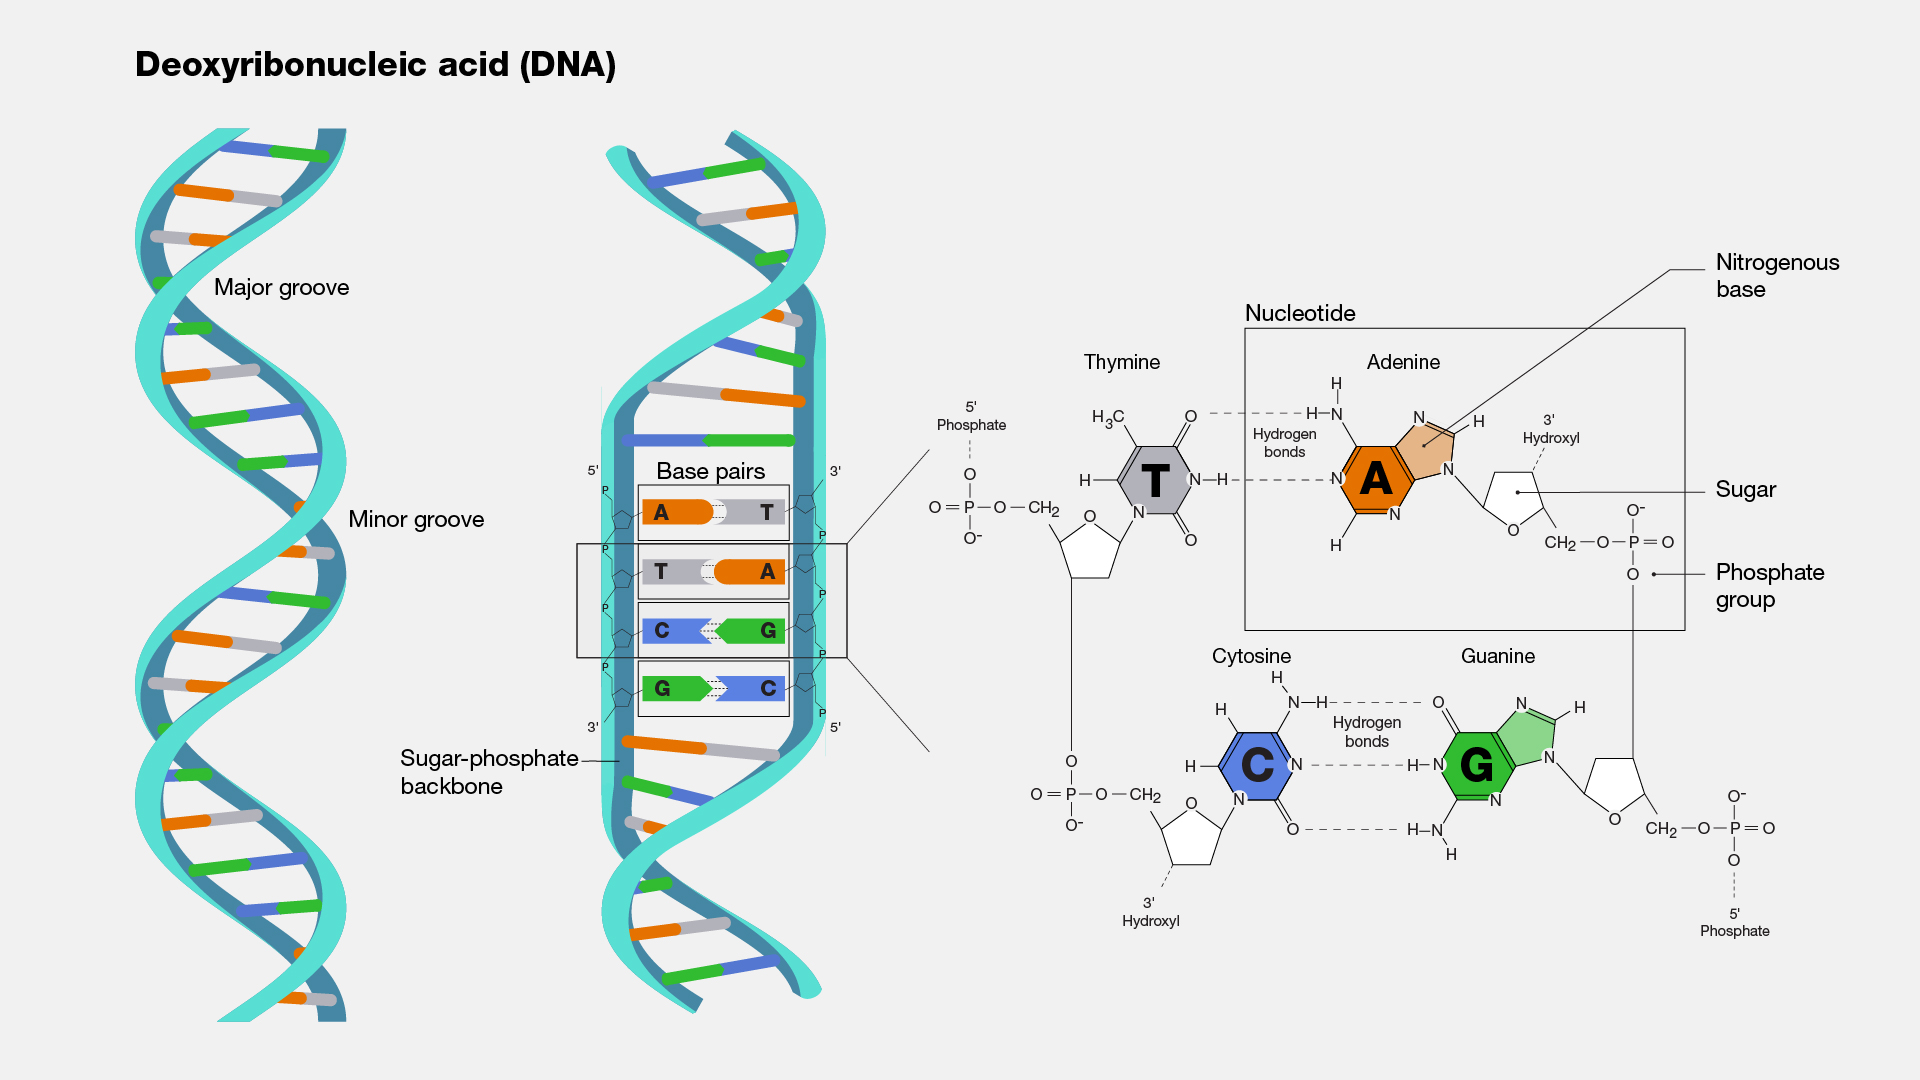
\includegraphics[width=0.6\textwidth]{dna.jpg}
  \caption{Structure of the \gls{dna} double helix}
  \label{fig:dna}
\end{figure}

The functional units of \gls{dna} are called genes, which are discrete
sequences that contain the instructions for producing proteins. However,
\gls{dna} itself cannot participate directly in protein synthesis. Instead, a
process called transcription is used to copy the information from a gene to a
\gls{rna} molecule as seen in \textcite{basic_biology_NCBI2002}. Unlike
\gls{dna}, \gls{rna} is single-stranded and uses uracil (U) instead of thymine
as one of its bases.

Among the various types of \gls{rna}, the best known is messenger \gls{rna}
(mRNA), which serves as an intermediary between genes and proteins. During
transcription, an mRNA molecule is synthesized as a complementary copy of a
gene, and this mRNA carries the genetic message from the \gls{dna} in the
nucleus to the ribosomes in the cytoplasm, where protein synthesis occurs. This
process, known as translation, is where the mRNA sequence is read in triplets
(called codons), each of which corresponds to a specific amino acid
\cite{central_dogma_molecular}.

%melhorar estrutura da imagem para ser como no paper
\begin{figure}[h]
  \centering
  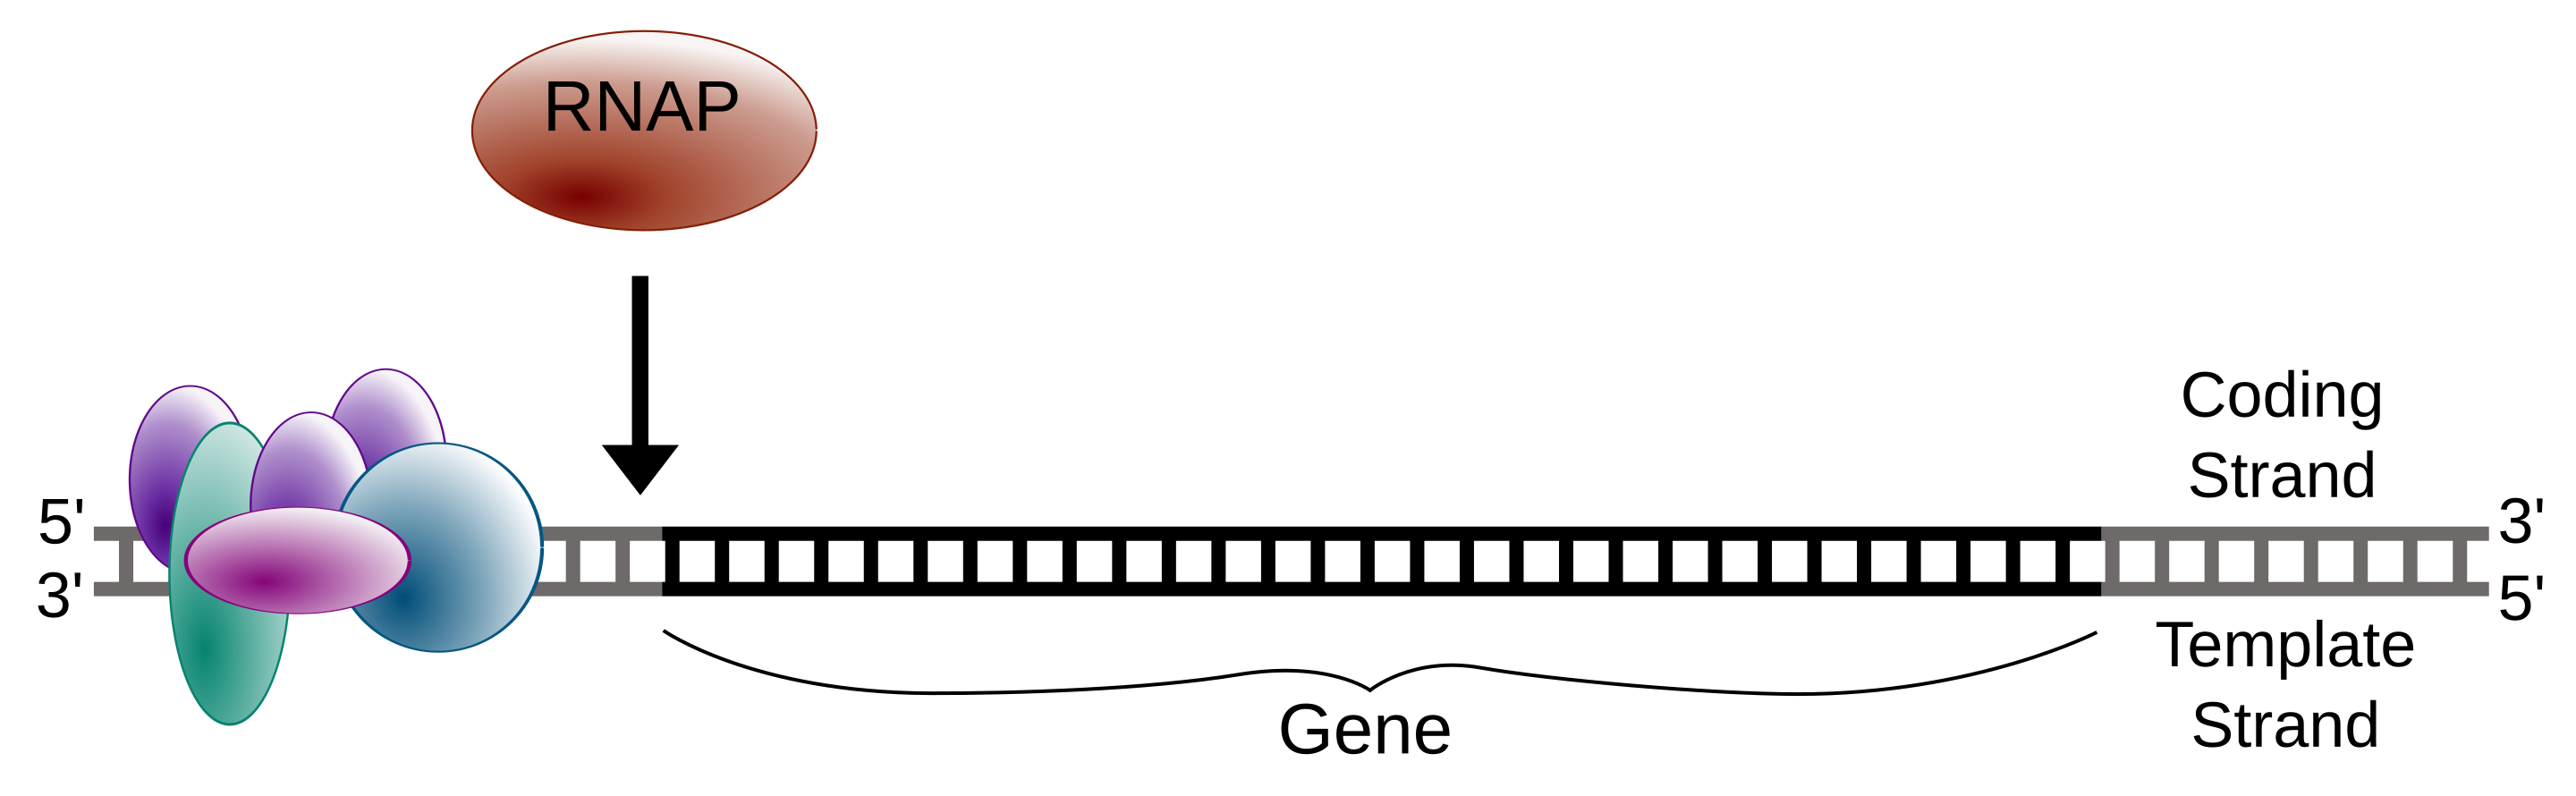
\includegraphics[width=0.3\textwidth]{transcription1.png}
  
\includegraphics[width=0.3\textwidth]{transcription2.png}
  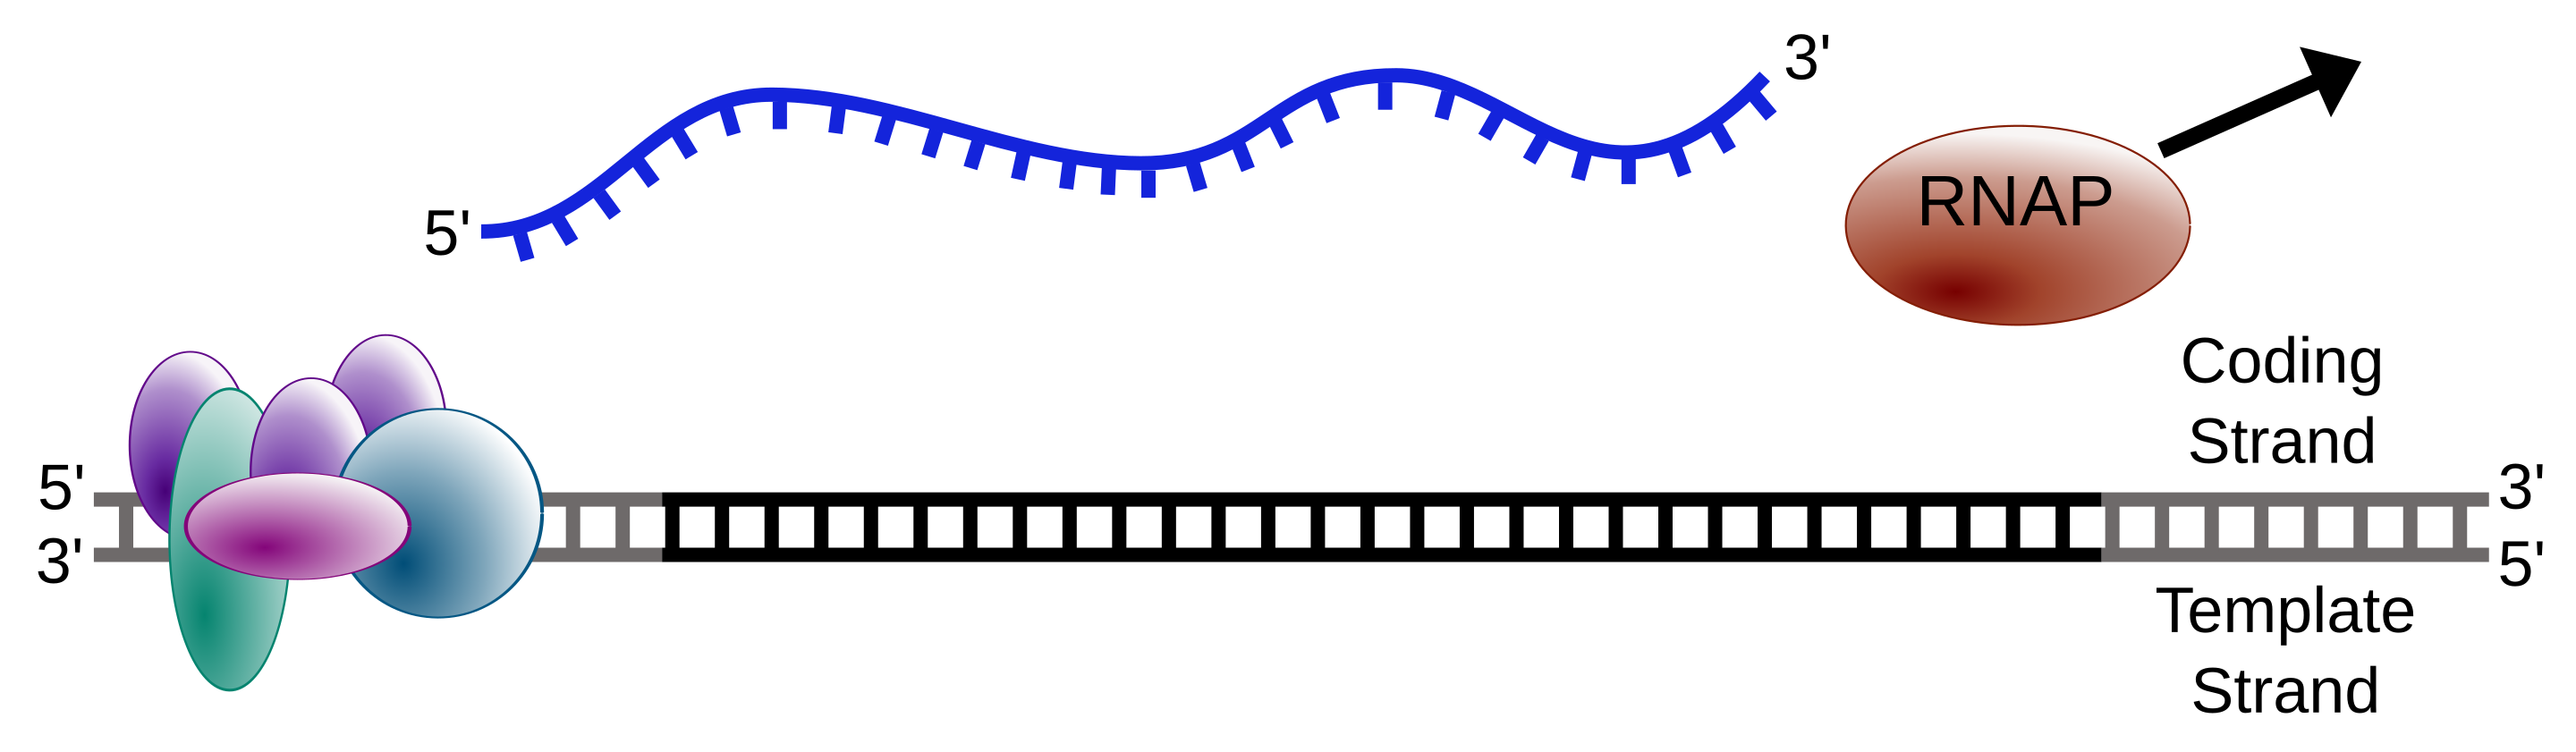
\includegraphics[width=0.3\textwidth]{transcription3.png}
  \caption{Illustration of the transcription mechanism: (a) initiation, (b) elongation, and (c) termination}
  \label{fig:transcription}
\end{figure}

The set of rules by which the nucleotide sequence in messenger \gls{rna} is
translated into a sequence of amino acids is known as the genetic code. This
code is composed of triplets of nucleotides, called codons, where each codon
specifies one of the twenty standard amino acids used in protein synthesis seen
in \textcite{genetic_codeNovozhilov2008O} study.

The genetic code is described as redundant but unambiguous. Redundancy means
that most amino acids are encoded by more than one codon—for example, leucine
is specified by six different codons—which provides a certain degree of
robustness to the system. At the same time, the code is unambiguous because
each codon corresponds to only one amino acid; that is, a given codon does not
encode multiple amino acids \cite{ConceptsBiology_DNA}.

Another fundamental characteristic of the genetic code is its universality.
With very few exceptions, the same codons specify the same amino acids in
virtually all living organisms, from bacteria to humans. This evolutionary
conservation has been fundamental in enabling the development of many molecular
biology tools and biotechnological applications prooved by
\textcite{genetic_codeKoonin2017}.

Although the focus of molecular biology for decades has been on the coding
sequence of the genome—that is, the genes that give rise to proteins—it is now
known that a large part of the human genome is transcribed into \gls{rna} that
does not code for proteins. These non-coding \gls{rna} (ncRNA) molecules play
crucial regulatory roles in controlling gene expression. One of the most
studied groups within this class are microRNAs (miRNAs), which appear to be
central elements in the fine-tuning of the genetic regulation process.

\subsection{MicroRNAs - The Regulators of Gene Expression}
MicroRNAs (miRNAs) are small non-coding \gls{rna} molecules, approximately $20$
to $25$ nucleotides in length, that play a key role in regulating gene
expression at the post-transcriptional level
\cite{regulatory_mecha_mirnaGulyaeva2016,
  first_mirna_Ambros1993,post_transcript_wightman1993}. Instead of encoding
proteins, miRNAs act by controlling the production of proteins from genes.

\begin{figure}[h]
  \centering
  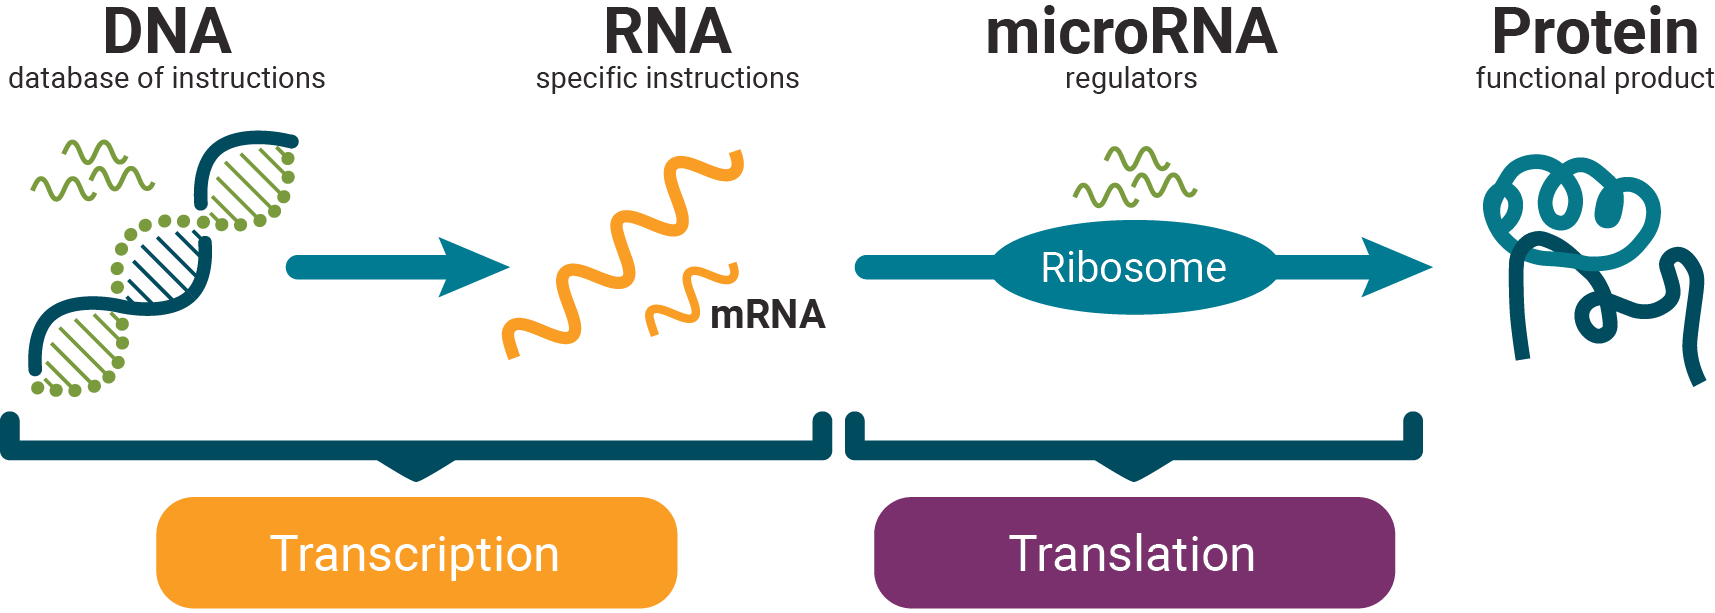
\includegraphics[width=0.8\textwidth]{mirna_process.png}
  \caption{The figure shows the process of gene expression: DNA is transcribed
    into mRNA, which is then translated into protein by the ribosome. microRNAs
    are shown as regulators acting on the mRNA before translation.}
  \label{fig:mirna_mechanism}
\end{figure}

In simple terms, \textbf{miRNAs function as molecular switches that bind to
  messenger \gls{rna} (mRNA) molecules}, blocking their translation into protein
or promoting their degradation. This mechanism depends on the degree of
complementarity between the miRNA sequence and that of the target mRNA:

\begin{itemize}
  \item When there is high complementarity, the mRNA tends to be degraded;
  \item When complementarity is partial, the miRNA generally acts by inhibiting
        translation without destroying the mRNA.
\end{itemize}

A study made by \textcite{role_mirna_Calaf2023} demonstrates the high
effienciency of this mechanism of regulation: a \textbf{single miRNA can
  control dozens to hundreds of different genes}, and it is estimated that more
than $60\%$ of human coding genes are targeted for regulation by miRNAs.

Due to this broad regulatory capacity, miRNAs play a central role in multiple
cellular processes such as proliferation, differentiation, apoptosis, and
stress response. Consequently, changes in miRNA expression profiles are
associated with several diseases, including cancer, neurodegenerative and
cardiovascular diseases. In an oncological context, miRNAs can act as oncogenes
(promoting tumor growth) or as tumor suppressors, depending on the biological
context and cell type as shown by
\textcite{regulatory_mecha_mirnaGulyaeva2016}.

Due to their specificity, stability, and direct involvement in relevant
molecular mechanisms, miRNAs have been extensively investigated as promising
biomarkers for diagnosis, prognosis, and subtype stratification in various
diseases—including cancer.

\subsection{Cancer - A Complex Disease}
Cancer is a disease characterized by the uncontrolled proliferation of
transformed cells, which can invade neighboring tissues and spread to other
parts of the body through processes such as metastasis. This definition, based
on \textcite{NCI2021,def_of_cancer_Brown2023}, has recently been expanded to
recognize the role of natural selection in the evolution of cancer: it is a
cellular system that continuously evolves, adapting to internal and external
pressures to ensure its survival.

Under normal conditions, the body's cells divide only when necessary, die when
damaged or obsolete, and are replaced by new ones. However, in cancer, this
biological balance is disrupted: abnormal cells gain the ability to multiply
independently of the body's signals and to resist programmed cell death
(apoptosis). These transformed cells become autonomous units that not only
ignore normal growth controls but also interact with the tumor microenvironment
to promote their own survival, using angiogenesis, immune evasion, and other
adaptive mechanisms \cite{def_of_cancer_Brown2023,NCI2021}.

The result is a heterogeneous cell population, subject to natural selection
within the human body. Cells that acquire adaptive advantages (e.g., higher
proliferation rate, drug resistance, or migration ability) tend to prevail,
making cancer a constantly evolving disease \cite{def_of_cancer_Brown2023}.

Although cancer can arise in virtually any tissue, not all cellular changes are
malignant. There are precancerous conditions, such as \textit{hyperplasia or
  dysplasia}, which represent an increase in the number of cells or changes in
their morphology, but which do not yet invade surrounding tissues.

Progression of cancer is a complex process that involves the
\textbf{acquisition of invasive and metastatic capacity—properties that
  distinguish malignant tumors from benign ones}. This process can be silent for
years, until more severe symptoms arise, often related to the invasion of vital
organs.

\subsection{Breast Cancer \& its Subtypes}

Breast cancer is the most commonly diagnosed cancer in women worldwide and is
one of the leading causes of cancer death in developed and developing countries
as seen in \textcite{BreastEpidemiology_Romanowicz2022,
  updatedbca_Hong2022Breast}. It is estimated that \textbf{one in eight women}
will be diagnosed with this disease during their lifetime, although it can also
affect men—albeit with a much lower incidence.

Most breast tumors are originated in the epithelial cells of the ducts or
lobules of the breast, which acquire malignant properties after the
accumulation of genetic and epigenetic changes. These events alter the normal
control of cell proliferation, differentiation, and apoptosis, allowing for
unregulated tumor growth \cite{origins_and_evolution_bca_Polyak2007}.

\begin{figure}
  \centering
  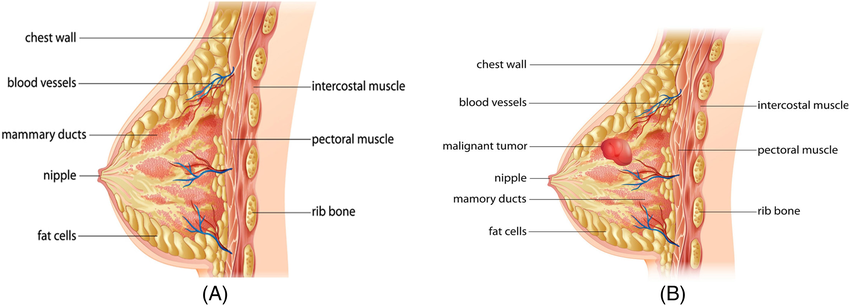
\includegraphics[width=0.8\textwidth]{bca_anatomy.png}
  \caption{In (A) we have a normal breast tissue, while in (B) we can see
    the presence of a malignant tumor \cite{bca_anatomy_figure_Muthu2020}.}
  \label{fig:breast_cancer_anatomy}
\end{figure}

The development of the disease is associated with a set of well-established
risk factors, which include:
\begin{itemize}
  \item Age and family history of the disease;
  \item Hereditary genetic mutations, especially in the \textit{BRCA1} and
        \textit{BRCA2} genes;
  \item Prolonged exposure to endogenous or exogenous hormones (e.g., early menarche,
        late menopause, hormone therapy);
  \item Environmental and behavioral factors, such as obesity, physical inactivity,
        alcohol consumption, and a diet rich in saturated fats
        \cite{BreastEpidemiology_Romanowicz2022,clinical_implication_bca_Adamo2015}.
\end{itemize}

From a molecular and clinical point of view, \textbf{breast cancer is highly
  heterogeneous}. Each tumor may have unique combinations of genetic alterations,
signaling pathways, and gene expression profiles, which are reflected in
different clinical behaviors, degrees of aggressiveness, and response to
treatment
\cite{origins_and_evolution_bca_Polyak2007,diff_bca_usa_Howlader2018}.

Early detection is crucial for prognosis. When diagnosed in its early stages,
breast cancer has survival rates of over $90\%$. However, in more advanced
stages, especially when metastases appear, controlling the disease becomes
substantially more difficult and the therapeutic goal shifts from curative to
palliative \cite{updatedbca_Hong2022Breast,clinical_implication_bca_Adamo2015}.

The therapeutic approach is typically multimodal, combining surgery,
radiotherapy, chemotherapy, hormone therapy, and targeted or biological
therapies, depending on the characteristics of the tumor and the patient's
general condition. The most significant advance in the last decade has been the
transition from a uniform model to a personalized treatment approach, tailored
to the molecular subtype and individual risk as studied by
\textcite{BreastEpidemiology_Romanowicz2022}.

In addition, a study made by \textcite{origins_and_evolution_bca_Polyak2007}
recognized that breast tumors are not static entities. Due to phenomena of
intra-tumor heterogeneity and clonal evolution, tumors adapt to the selective
pressure of treatments, often leading to the development of therapeutic
resistance and disease progression.

Given the molecular complexity and clinical diversity of breast tumors, it was
established in the papers
\textcite{clinical_implication_bca_Adamo2015,bc_subtypes_Prat2015Clinical} that
breast cancer is not a single disease but rather a collection of biologically
distinct entities that arise from a common anatomical site. This heterogeneity
is reflected in major differences in tumor progression, metastatic behavior,
response to therapy, and long-term prognosis.

To better capture this complexity and inform clinical decision-making,
researchers from various studies, such as
\textcite{bc_molecular_Perou2000,bc_subtypes_Prat2015Clinical}, have developed
a molecular classification system that subdivides breast tumors into intrinsic
subtypes. These subtypes are defined based on the expression status of three
key biomarkers: \textbf{estrogen receptor (ER)}, \textbf{progesterone receptor
  (PR)}, and \textbf{human epidermal growth factor receptor 2 (HER2)} as well as
other proliferation indices (e.g., Ki-67) and gene expression patterns. This
classification underpins modern precision oncology approaches and has profound
implications for therapy and prognosis.

As shown in the table \ref{tab:bc_subtypes_summary}, breast cancer can be
classified into four main intrinsic subtypes based on the expression of these
biomarkers and other molecular characteristics:

%%% REMOVER O h para !t no final1!!!!!!asdonasodniasoindaosindoi
\renewcommand{\arraystretch}{1.3}
\begin{table}[h]
  \centering
  \small
  \caption{Summary of intrinsic breast cancer subtypes and typical characteristics of each one.\newline\textit{References:} \cite{clinical_implication_bca_Adamo2015}, \cite{diff_bca_usa_Howlader2018}, \cite{bc_subtypes_Prat2015Clinical}, \cite{updatedbca_Hong2022Breast}, \cite{tnbc_therapies_Mahalingam2020The}.}
  \label{tab:bc_subtypes_summary}
  \begin{tabularx}{\textwidth}{l l l l X}
    \toprule
    \textbf{Subtype}  & \textbf{Receptors / HER2} & \textbf{Prolif.} & \textbf{Prognosis} & \textbf{Treatment}          \\
    \midrule
    Luminal A         & ER+/PR+, HER2−            & Low              & Favorable          & Endocrine only              \\
    \midrule
    Luminal B         & ER+, PR↓, HER2±           & High             & Intermediate       & Hormone ± Chemo ± Anti-HER2 \\
    \midrule
    HER2-enriched     & HER2+, ER−, PR−           & High             & Improved           & Anti-HER2 + Chemo           \\
    \midrule
    Basal-like / TNBC & ER−, PR−, HER2−           & High             & Poor               & Chemo; ± PARP/IO (selected) \\

    \bottomrule
  \end{tabularx}

  \vspace{1ex}
  \raggedright
  \footnotesize
  \textit{Acronyms:} Chemo = Chemotherapy , IO = Immunotherapy .
\end{table}

Recent evidence by
\textcite{intratumor_heterogeneity_Yeo2017,origins_and_evolution_bca_Polyak2007}
suggests that multiple subtypes can coexist within the same tumor (a phenomenon
called intra-tumor heterogeneity). This complexity contributes to therapeutic
resistance and disease progression.

\subsection{Nucleic acids as gene therapies}
\label{sec:nucleic_acids_gene_therapies}
% Now that we have a better understanding of limitations that most of cancer treatments 
% have, \gls{mirna} have emerged as a promising tool in the field of cancer
% research and treatment. 

% Considering them as the "natural regulators" of the human body, we can leverage 
% that regulating mechanism and use it to 

\newpage
\section{Related work}

This section will present a critical review of computational approaches
developed to date to explore the potential of \gls{mirna} as biomarkers in the
context of oncology, covering both \gls{bc} and other malignant neoplasms. The
contributions of \gls{ml} and \gls{dl} models applied to the task of
classifying different cancer subtypes will also be analyzed, with a special
focus on methodologies that integrate molecular data with data from other
nature, like clinical characteristics for example.

\gls{ml}, a branch of \gls{ai}, involves
developing computational models that learn from data to make predictions or
decisions. These models are typically trained using either supervised
learning, where the target outcomes are known and used during training, or
unsupervised learning, in which no explicit labels or outcome variables are
provided. In both paradigms, the goal is to uncover meaningful patterns in the
data that can be used to generate predictive insights, such as detecting the
presence of cancer, estimating survival probabilities, or stratifying patients
into risk categories. \gls{ml} techniques are particularly valuable when dealing with
unstructured or complex clinical datasets, as is often the case in oncology.

In recent years, the application of \gls{ml} algorithms to the field of
biomedicine has led to significant advances in the analysis of complex and
high-dimensional data, including the expression of \gls{mirna} in cancer
\cite{role_of_ai_giger2021}. In this context, several studies have explored the
use of computational models for the classification of tumor subtypes and/or the
identification of discriminative biomarkers, with promising results but also
with important limitations.

In this context, we will review and analyze scientific works that have
leveraged \gls{ml} algorithms in contexts similar to the stratification of
\gls{bc} subtypes based on \gls{mirna} expression profiles, complementing them
with data of other types (multi-omics data). For each study, it will be
important to define the specific work in question so that we can analyze the
methodology, algorithms used, and results obtained, all based on the specific
context of the research in question, in order to capture and consolidate a
ground on which we can work. At the end of the review, we will discuss how
these contributions inform and substantiate the methodological choices made in
the present work, justifying, whenever possible, the algorithmic and
experimental choices based on the available scientific evidence.

\subsection{Leveraging \gls{ai} models for \gls{bc} subtype classification}
% HERE: começar com cancer classification em geral -> depois falar de 
% Papers a usar: 4, 10 , 11, 12 ( estes dois últimos são com imagens, mas podemos abordar)

The classification of different types of cancer using computational models has
been one of the most explored areas within the application of \gls{ai} to
medicine. Let's take a look at the work of
\textcite{ai_in_dermacancer_esteva2017}, a remarkable advance in this “new”
relationship between computers and dermatology, where deep neural networks
(Figure \ref{fig:DNN}) have demonstrated capabilities comparable to those of
human experts in the diagnosis of malignant skin lesions.

\begin{figure}[htbp]
  \centering
  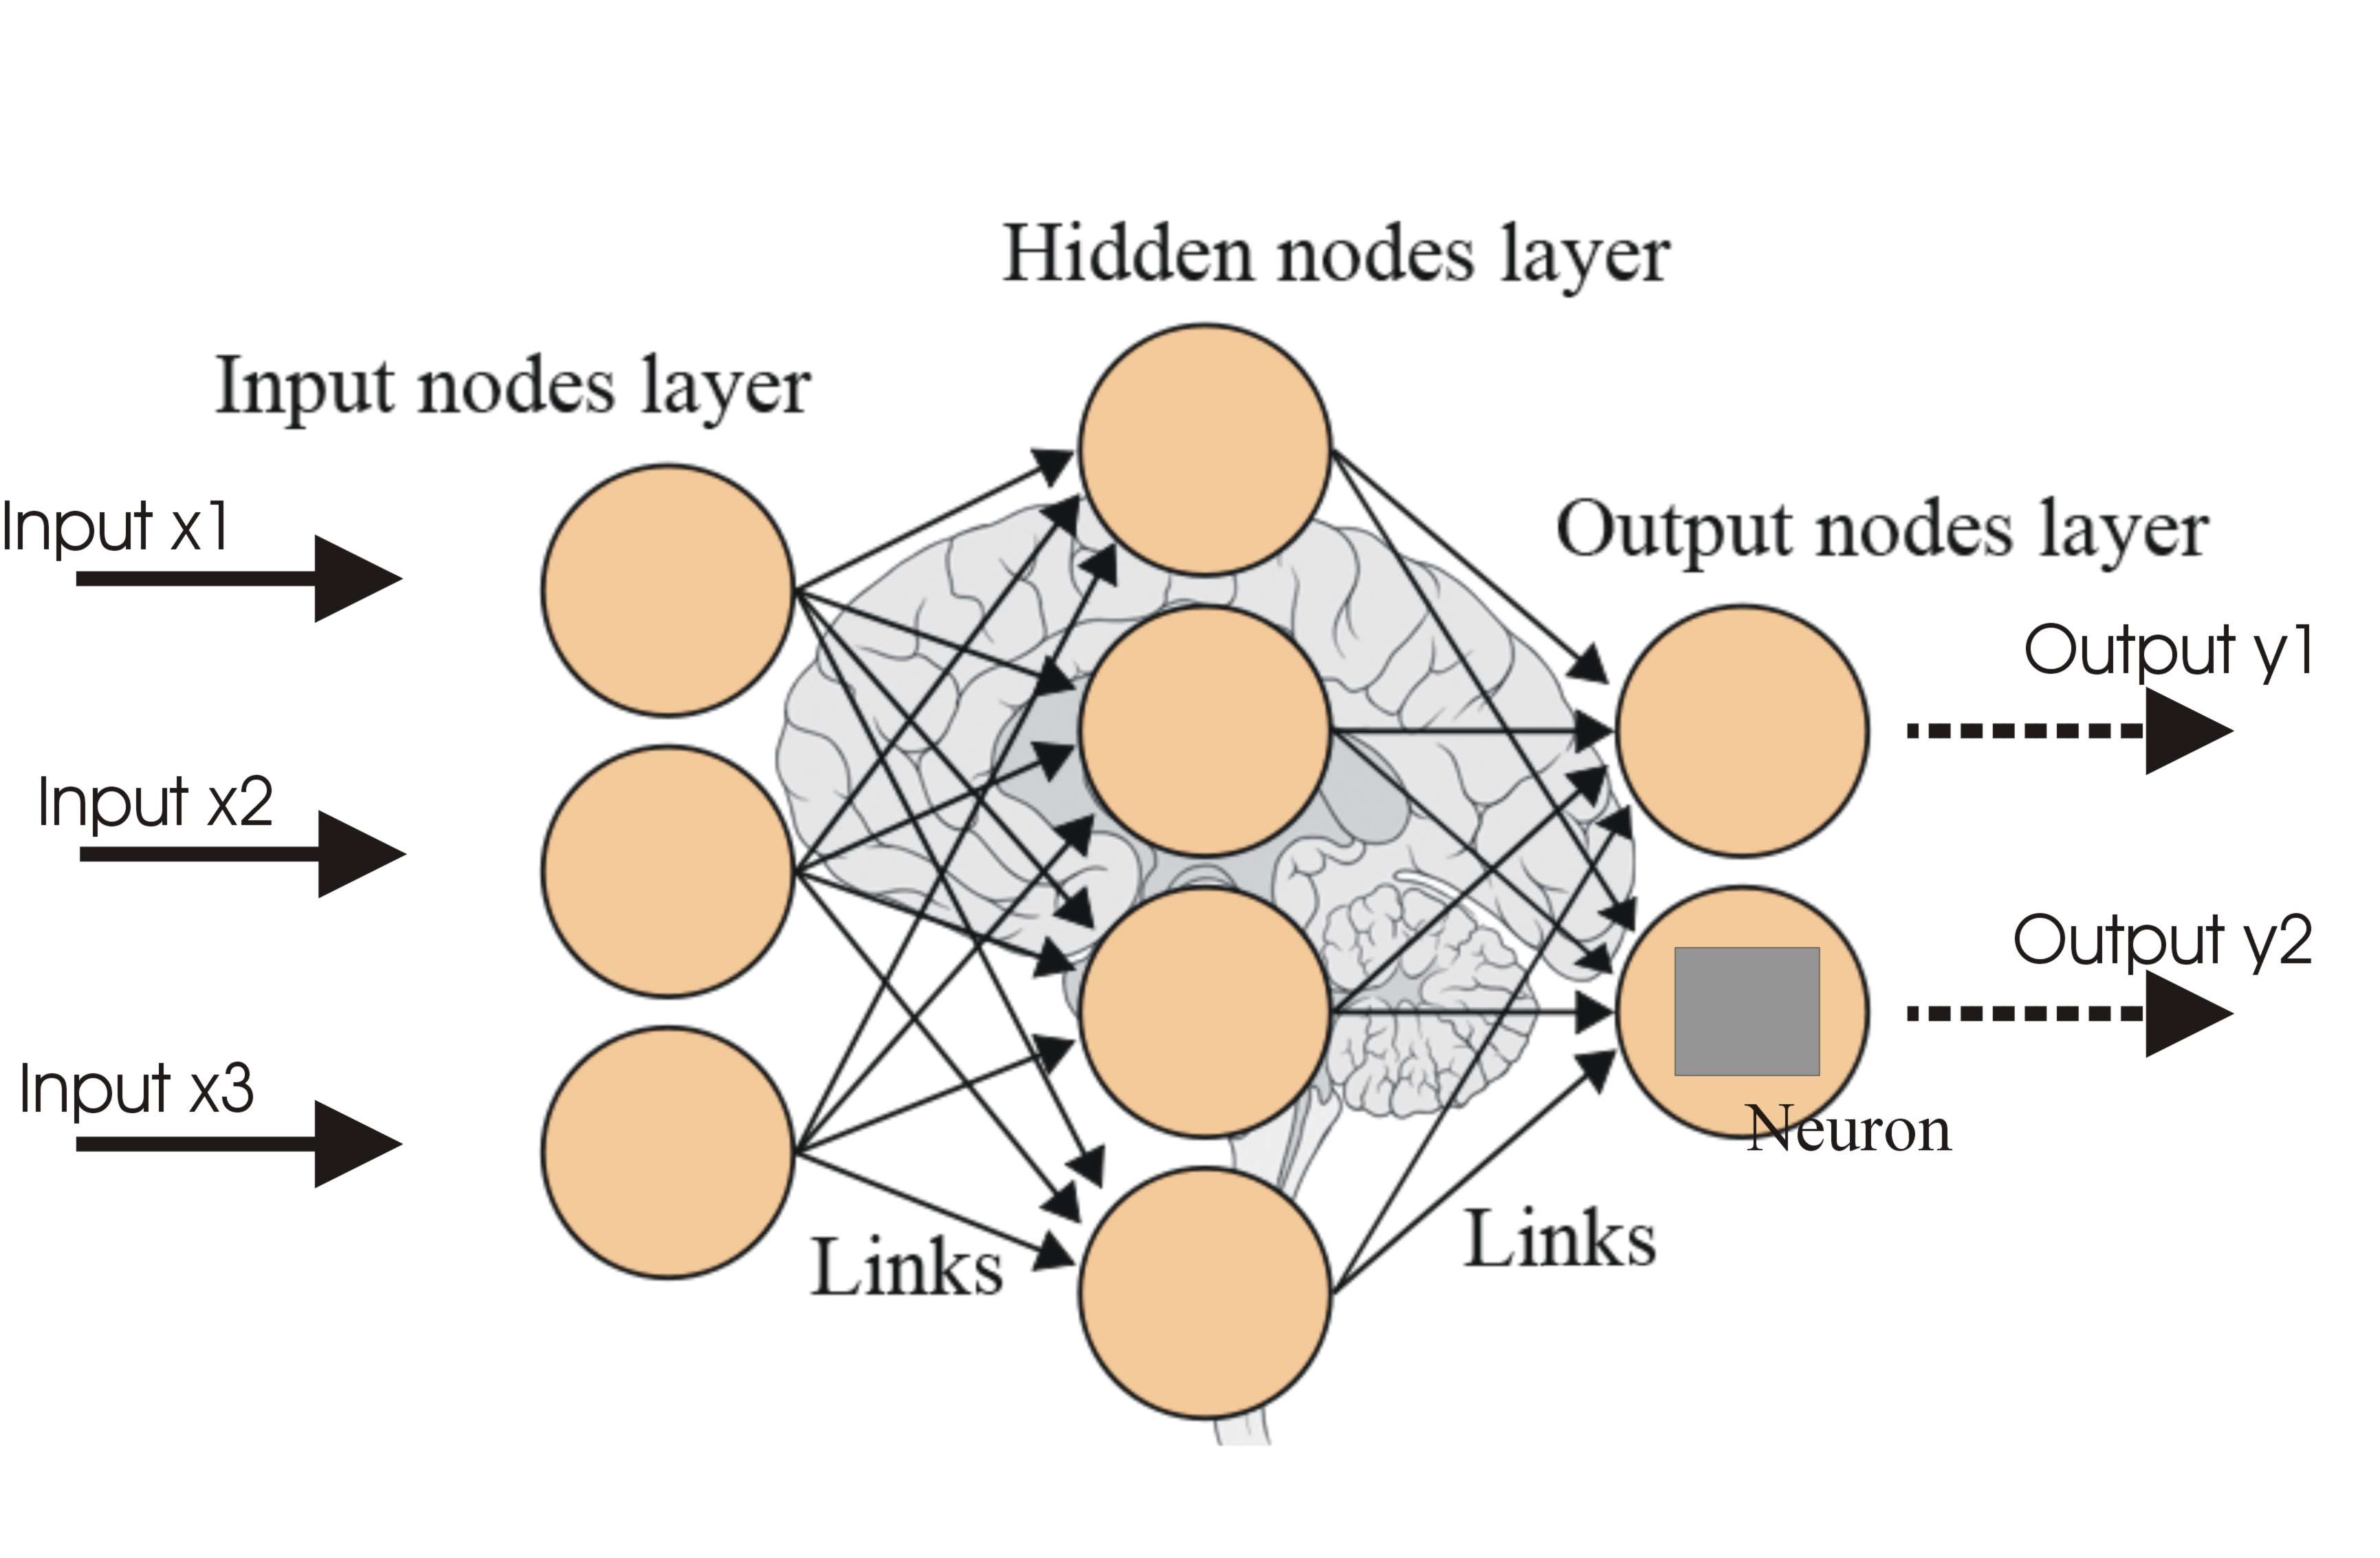
\includegraphics[width=0.7\textwidth]{/Users/JoseRomano/Documents/Tese/bca-thesis/Chapters/Figures/NN.png}
  \caption{Structure of an deep neural network (DNNs). It shows the input, hidden, and output layers, with connections between neurons responsible for processing information.}
  \label{fig:DNN}
\end{figure}

This work was made possible by the use of an architecture based on
convolutional neural networks (CNNs) - a type of DNN that is particularly
effective in image processing (Figure \ref{fig:CNN_derma}). CNNs work by
applying convolutional filters that extract visual patterns at different levels
of complexity, allowing the model to identify relevant features directly from
the image pixels, without the need for specialized preprocessing.

\begin{figure}[htbp]
  \centering
  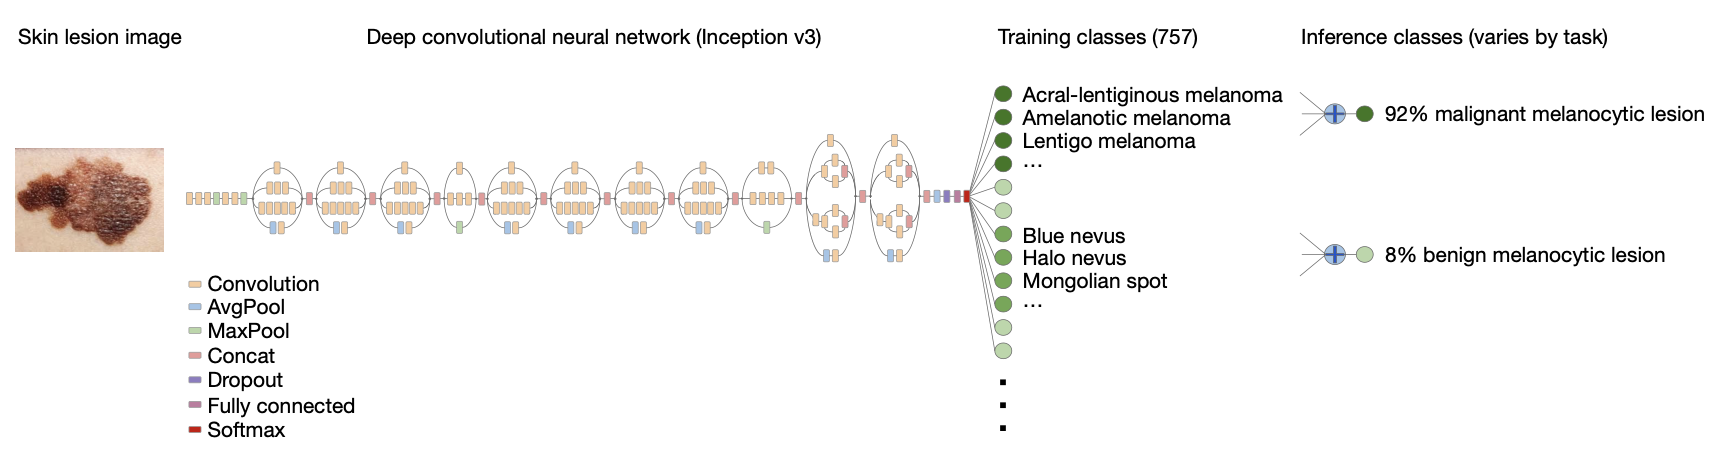
\includegraphics[width=1.0\textwidth]{/Users/JoseRomano/Documents/Tese/bca-thesis/Chapters/Figures/CNN_derma.png}
  \caption{Schematic of the CNN used by \textcite{ai_in_dermacancer_esteva2017} with Inception v3 architecture, adapted to classify skin lesions based on clinical images. The network generates a probability distribution over clinical classes, based on a structured medical taxonomy.}
  \label{fig:CNN_derma}
\end{figure}

The biggest problem with this methodology is that these architectures require a
large number of cases (positive and negative) in order to learn the necessary
patterns. In this case, 129{,}450 clinical images covering more than 2{,}000
different diseases were used. Some factors that determined the good results of
this model were:

\begin{enumerate}
  \item The photographic variability of the samples on which it was trained, since they
        covered not only images taken with mobile phones, but also dermoscopy images;

  \item The manipulation of images during training, enlarging and inverting them to
        increase the adaptability and robustness of the model;

  \item The use of a structured medical taxonomy (Figure \ref{fig:taxonomy}), built on
        clinical and visual criteria, which allowed for the organization of more than
        2{,}000 diseases into a hierarchy of 757 fine-grained training classes, such as
        \textit{acrolentiginous melanoma} and \textit{amelanotic melanoma}.
\end{enumerate}

\begin{figure}[htbp]
  \centering
  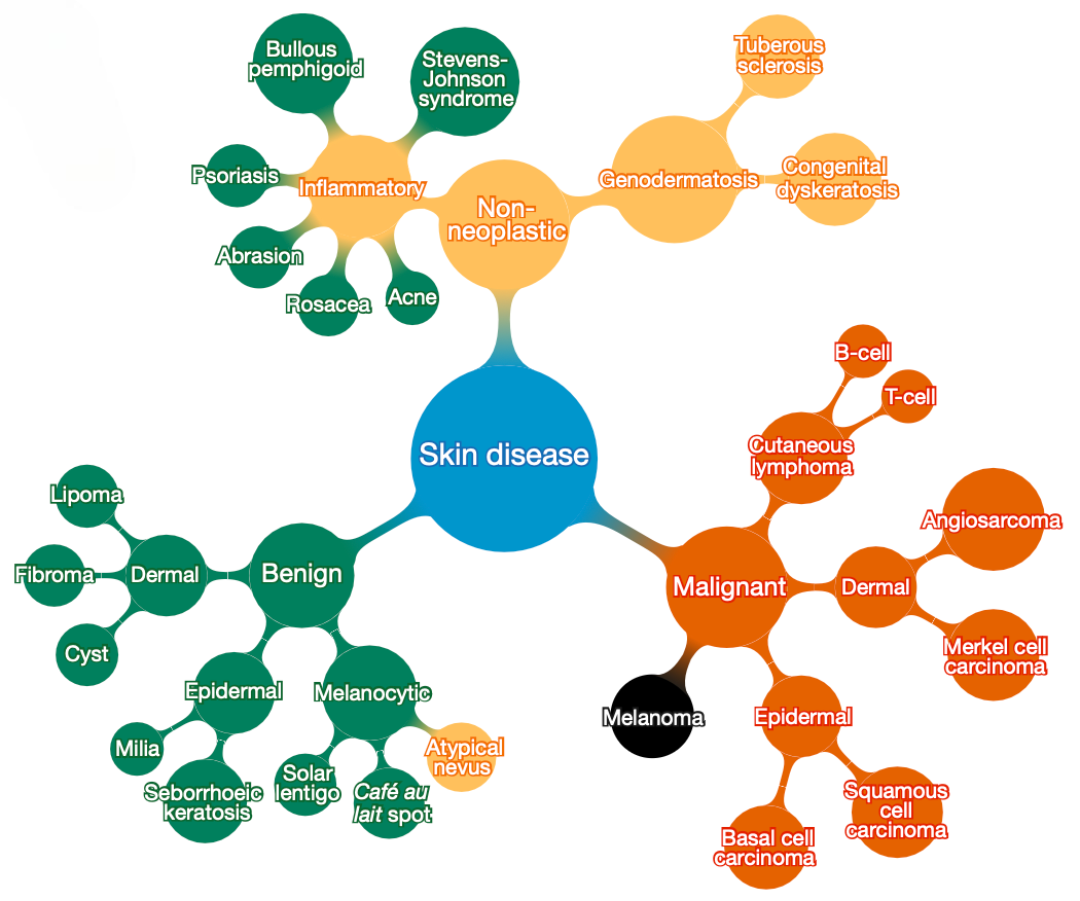
\includegraphics[width=0.5\textwidth]{/Users/JoseRomano/Documents/Tese/bca-thesis/Chapters/Figures/taxonomy.png}
  \caption{A subset of the hierarchical taxonomy developed in the study by \textcite{ai_in_dermacancer_esteva2017}, with diseases organized by clinical and visual similarity into three major groups: benign, malignant, and non-neoplastic.}
  \label{fig:taxonomy}
\end{figure}

The result? A computational model that not only achieved performance comparable
to that of certified dermatologists, but in several scenarios even demonstrated
superiority over average human performance, verifiably by this confusion matrix
(Figure \ref{fig:conf-matrix-docs}). The trained convolutional neural network
was able to classify two critical clinical cases with high accuracy:
keratinocytic carcinomas versus benign seborrheic keratoses, and malignant
melanomas versus benign nevi. In these binary scenarios, it obtained areas
under the curve (\textit{AUC}) of 0.96 and 0.94, respectively (Figure
\ref{fig:AUC_dnn_model}) - values higher than those obtained by dermatologists
in the same tasks. \textit{AUC} is a metric that quantifies a model's ability
to distinguish between classes, with values close to 1 indicating excellent
performance.

\begin{figure}[htbp]
  \centering
  \begin{subfigure}[b]{0.45\textwidth}
    \centering
    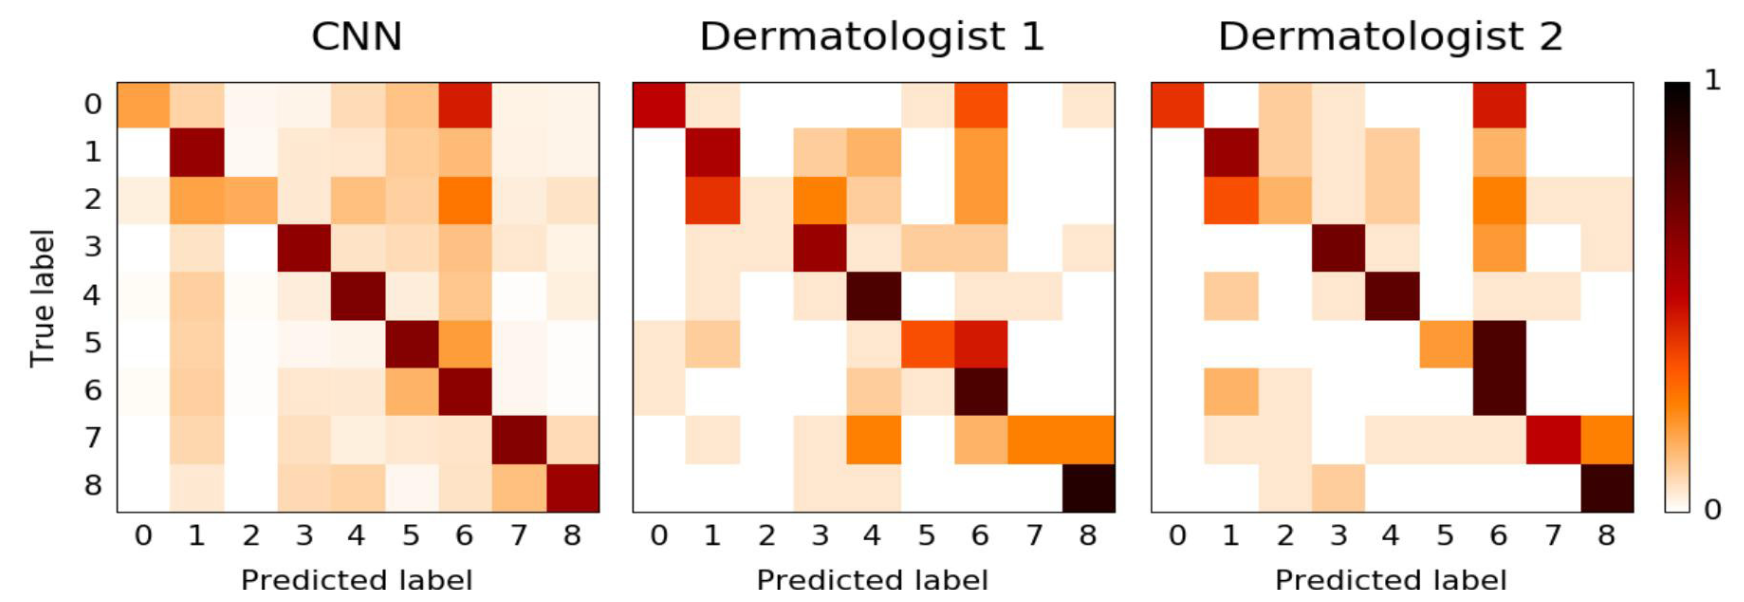
\includegraphics[width=\textwidth]{/Users/JoseRomano/Documents/Tese/bca-thesis/Chapters/Figures/conf-matrix-docs.png}
    %\caption{(a)}
    \label{fig:conf-matrix-docs}
  \end{subfigure}
  \hfill
  \begin{subfigure}[b]{0.45\textwidth}
    \centering
    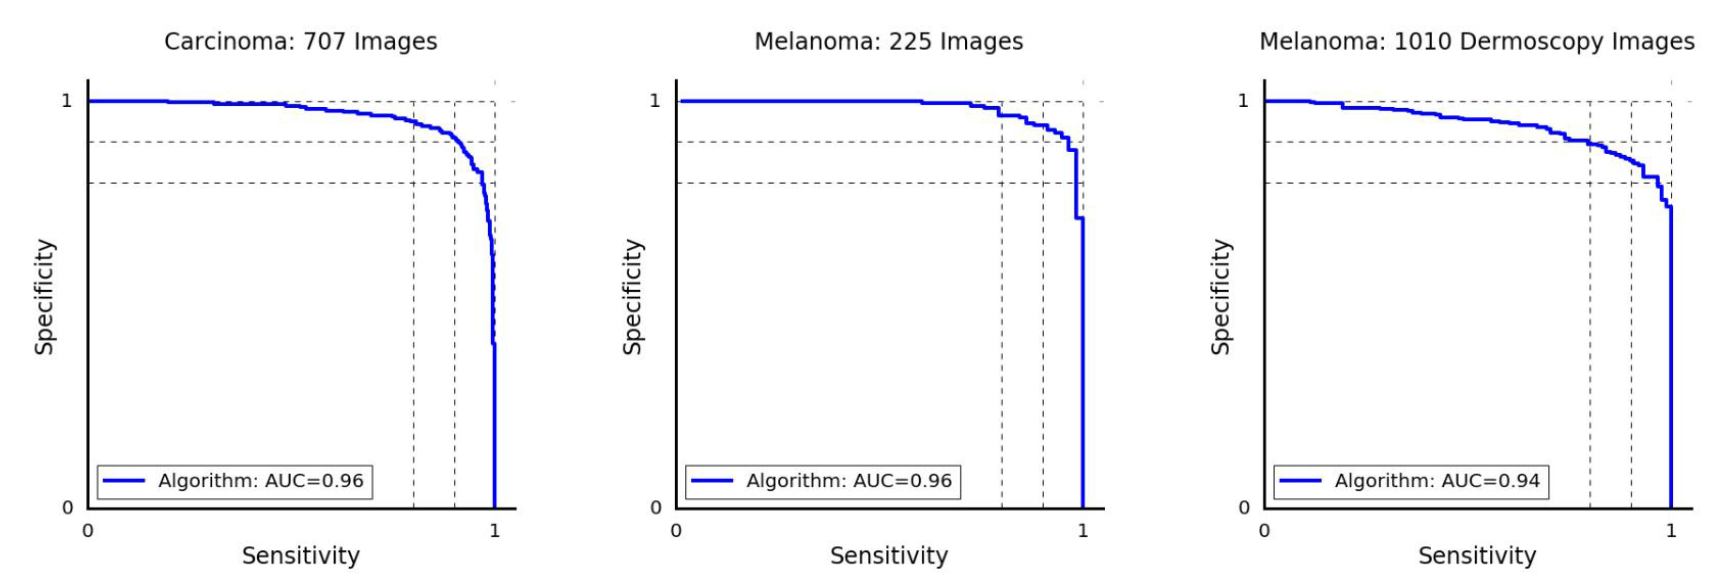
\includegraphics[width=\textwidth]{/Users/JoseRomano/Documents/Tese/bca-thesis/Chapters/Figures/AUC_derma_2.png}
    %\caption{(b)}
    \label{fig:AUC_dnn_model}
  \end{subfigure}
  \caption{Performance evaluation of the convolutional neural network (CNN) in skin lesion classification. (a) Confusion matrices of CNN and two dermatologists. The concentration on the diagonal indicates correct classifications; CNN shows less dispersion and better overall performance \cite{ai_in_dermacancer_esteva2017}. (b) Reliability of the CNN demonstrated by \textit{AUC} curves on a larger, independent dataset \cite{ai_in_dermacancer_esteva2017}.}
  \label{fig:AUC_derma_total}
\end{figure}

Furthermore, in more complex scenarios with multiple classes (three and nine
disease categories), the model maintained \textbf{remarkable levels of
  accuracy} (72.1\% and 55.4\%), surpassing or equaling human experts. The
robustness of the methodology, that is, its ability to maintain performance
under different conditions or test data, was also confirmed in larger test
sets, where the network's performance remained stable, with \textbf{minimal
  variations in evaluation metrics}. From a technical standpoint, it was an
efficient, scalable system with \textbf{potential for application in mobile
  devices}, which gives it relevant clinical applicability, especially in
contexts with limited access to specialists.

Internal analyses further reinforced confidence in the model, showing that it
learned consistent clinical representations: the network tended to
\textbf{group diseases with similar visual characteristics} (Figure
\ref{fig:tsne_derma}) and focused its attention on the damaged areas of the
images, ignoring irrelevant regions such as background or healthy skin -
promising evidence of \textit{automated clinical focus} with real practical
utility.

\begin{figure}
  \centering
  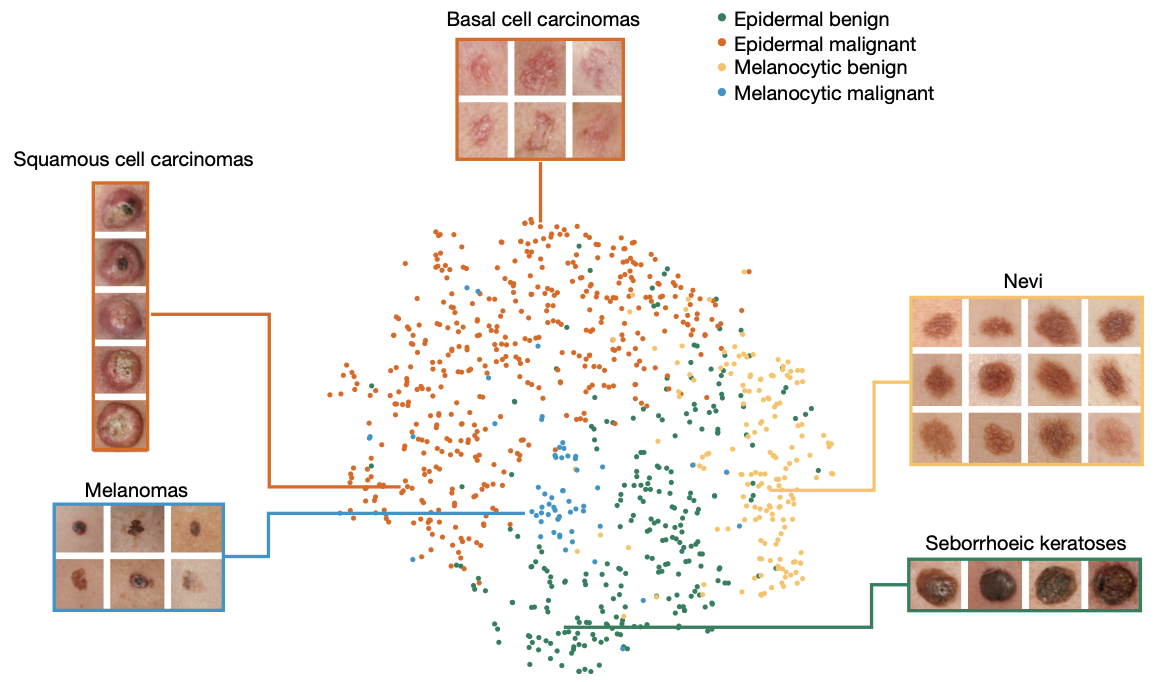
\includegraphics[width=\textwidth]{/Users/JoseRomano/Documents/Tese/bca-thesis/Chapters/Figures/t_sne_derma.png}
  \caption{t-SNE projection of the internal representations of the last hidden layer of the CNN \cite{ai_in_dermacancer_esteva2017}. The different classes of lesions are grouped into distinct clouds, revealing the model's ability to extract relevant discriminative features.}
  \label{fig:tsne_derma}
\end{figure}

\subsection{\gls{ml} unravelling microRNAs as biomarkers}
% Papers a usar: 1, 2 e 3

\subsection{Comparison with thesis approach}
% Papers a usar: 2, 4 e 10

\subsection{Other relevant work}
% HERE: applying ml in diagnosis and prognosis + ai in oncological nanomedicine
% Papers a usar: 6,8,5,7

\subsection{Conclusion}